\documentclass[12pt,a4paper]{article}
\usepackage[utf8]{inputenc}
\usepackage[czech]{babel}
\usepackage[T1]{fontenc}
\usepackage{graphicx}
\usepackage{frcursive}
\usepackage{hyperref}
\usepackage{listings}
\usepackage{xcolor}
\usepackage{geometry}
\usepackage{mathptmx} % Times New Roman
\usepackage{setspace}
\newcommand{\setfont}[2]{{\fontfamily{#1}\selectfont #2}}
\onehalfspacing

\hypersetup{
    colorlinks=true,
    linkcolor=black,
    filecolor=magenta,      
    urlcolor=cyan,
}

\setlength{\parindent}{0pt}
\setlength{\parskip}{1em}

\begin{document}

% -----------------------------------------------------------------------------
% TITULNÍ STRANA
% -----------------------------------------------------------------------------
\thispagestyle{empty}

    \begin{minipage}[t]{0.5\textwidth}
    \includegraphics[width=120pt]{images/logo.png}
    \end{minipage}

    \vspace*{3cm}

\begin{center}
    {\Huge \textbf{Příprava slavnostní tabule pro 2 osoby}} \\[1cm]
    {\Large \textbf{Slavnostní hostina v rámci Křtin}} \\[2cm]
\end{center}

\vfill

\begin{flushleft}
        Název: \textbf{Samostatná odborná práce}\\
        Téma: \textbf{Slavnostní hostina v rámci Křtin}\\
        Název práce: \textbf{Příprava slavnostní tabule pro 2 osoby}\\
        Název školy: \textbf{Střední odborné učiliště a Střední odborná škola Žatec}\\
        Kód a název oboru vzdělávání: \textbf{65-42-M/01}\\
        Název zaměření: \textbf{Hotelnictví}\\
        Třída: \textbf{3. A}\\
        Školní rok: \textbf{2025/2026}\\
        Jméno a Příjmení žáka: \textbf{Tereza Kováčová}\\
\end{flushleft}

\newpage
\tableofcontents
\newpage

% -----------------------------------------------------------------------------
% 1. ÚVOD
% -----------------------------------------------------------------------------
\section{Úvod}
Dobrý den, vítám vás na slavnostní hostině. Jmenuji se Tereza Kováčová, jsem žákyně 3. ročníku soukromé střední a odborné školy hotelnictví a cestovního ruchu. V rámci mé praktické zkoušky jsem si pro Vás připravila slavnostní hostinu s názvem: \textbf{Slavnostní hostina v rámci Křtin}.

Toto téma je velmi známé, ale jeho hloubka zůstává často skrytá. Je to jeden z nejstarších a nejdůležitějších rituálů 1. století, kteří tvoří základ mnoha křesťanských církví a má kořeny hluboko v historii lidstva a dodnes představují slavnostní bránu do duchovního života.

Křest je vlastně rituál, ve kterém se člověk stává členem křesťanské komunity. Je to akt, při kterém je člověk ponořen nebo pokřtěn svěcenou vodou ve jménu Otce, Syna i Ducha svatého. Počátky křtu nespočívaly ve velkolepých chrámech, ale v drsném prostředí řeky Jordán, dnes se konají většinou v kostele.

Historie sahá až do doby Jana Křtitele, který křtil lidi na znamení pokání, připravujíc je na příchod Mesiáše. Již zde se projevila klíčová symbolika - voda jako očistný prvek smývající viny a připravující srdce k proměně. Obřad získal svou podobu, když ho přijal sám Ježíš Kristus. Jeho křest potvrdil důležitost rituálu. Křest se pak definoval z rituálu pokání na iniciační svátost. Křesťanství definuje křest jako prostředek, jímž je člověk očištěn, znovuzrozen a přijat.

Zatímco Církev křtila především dospělé, kteří se na akt museli dlouho připravovat, s nástupem středověku převážil křest dětí. V době vysoké dětské úmrtnosti se stalo prioritou zajistit dítěti spásu okamžitě po narození. S tímto přechodem se objevila instituce kmotrů, kteří se zavazují pomáhat s výchovou dítěte ve víře, čímž se rozšiřuje okruh slavících rodin.

Gastronomie vstupuje na scénu ve chvíli, kdy duchovní akt končí a začíná společenská oslava. Slavnostní hostina, která následuje po obřadu, je sekulárním vyjádřením radosti. Shromažďuje rodinu a přátele, aby společně oslavili nový život a nového člena komunity. Právě proto je tato událost důležitá pro gastronomii. Kombinuje tradici, eleganci a vysoké nároky na kvalitu servisu, které odpovídají vážnosti a zároveň radosti tohoto klíčového životního milníku.

Dnes vás tedy zvu, abyste odložili všechny starosti a položili se do pochopení a zjištění více informací o Křtinách. Přeji vám krásný požitek z dnešního večera.
\newpage
% -----------------------------------------------------------------------------
% 2. CHARAKTERISTIKA
% -----------------------------------------------------------------------------
\section{Řešení}
\subsection{Charakteristika zvolené příležitosti}
Křtiny představují pro gastronomický provoz specifickou a žádanou příležitost, která vyžaduje kombinaci elegance, rodinného tepla a precizní organizace. Akce se koná v salonku nebo oddělené části restaurace. Je nutné zajistit klid a diskrétnost obsluhy, jelikož se jedná o soukromou rodinnou událost.

\subsection*{Tradiční formát}
\begin{itemize}
    \item [-] Nejčastěji jde o 3 až 4 chodový banketní způsob obsluhy s precizní synchronizací vydávání pokrmů z kuchyně a perfektním servisem u stolu.
\end{itemize}

\subsection*{Nároky}
\begin{itemize}
    \item [-] Kvalitní inventář, látkové ubrousky a decentní květinová výzdoba. Prostírání musí být elegantní a čisté, bílé nebo pastelové barvy, použití křesťanské symboliky. Dárkový stůl musí být předpřipraven pro dary.
\end{itemize}

\subsection*{Pokrmy}
\begin{itemize}
    \item [-] Lehčí slavnostní menu, které zahrnuje například telecí, drůbeží, ryby a kvalitní suroviny, estetická příprava.
\end{itemize}

\subsection*{Formální a etiketní pravidla}
\begin{itemize}
    \item [-] \textbf{Obsluha a servis:} Diskrétní a pozorná obsluha. Jídlo se podává stylem menu, nikoli raut. Všechny chody se podávají přesně v daný čas, aby se zachovala plynulost akce.
    \item [-] \textbf{Dress code:} Hosté přicházejí ve slavnostním, často pastelových barvách. Obsluha musí mít dokonale čisté a upravené oblečení, které odpovídá slavnostnímu tématu.
    \item [-] \textbf{Přípitek:} První slavnostní přípitek provádí otec daného dítěte nebo jeden z kmotrů. Obsluha musí být připravena s připraveným šampaňským pro všechny hosty a nealko varianty pro děti a řidiče.
\end{itemize}

Křtiny tak dokonale ukazují schopnost gastronomického provozu zvládnout komplexní a náročné, ale vysoce ziskové rodinné akce.
\newpage

% -----------------------------------------------------------------------------
% 3. MENU
% -----------------------------------------------------------------------------
\subsection{Sestavení menu}  


\begin{center}

Kanapka s parmskou šunkou a melounem\\
\vfill  
Bruschetta s rajčaty a mozzarellou\\
\vfill
Dýňové raviolky\\
\vfill
Hovězí vývar s játrovými knedlíčky\\
\vfill
Kuřecí roláda na bylinkách s pečenými bramborami ve slupce\\
\vfill
Vanilkové cupcakes\\
\vfill
\end{center}    

---------------------------------------------------------------------------------------------------------
\begin{center}
Rosé z Tavel (Francie)\\
\vfill
Pinot Noir (Francie)\\
\vfill
Veltínské zelené (Jižní Morava, Mikulov)\\
\vfill
Cabernet Sauvignon (Francie)\\
\vfill
Mozart Chocolate Coffee\\
\vfill
Prosecco extra dry \\
\end{center}

\newpage

% -----------------------------------------------------------------------------
% 4. OBJEDNÁVKA SLAVNOSTNÍ HOSTINY
% -----------------------------------------------------------------------------
\subsection{Objednávka slavnostní hostiny}

Slavnostní hostina v rámci křtiny\\
Tereza Kováčová\\
Dvořáková 31\\
431 01 Žatec\\

Restaurace U Tellerů\\
Růžová 42, Praha 4\\
203 74 Praha
\begin{flushright}
    V Praze dne 16. ledna 2026
\end{flushright}
Vážený vedoucí restaurace U Tellerů,\\
Ráda bych si u vás objednala slavnostní hostinu. Jedná se Křtiny mého malého bratrance.
Křtiny se uskuteční 15.4 2026 v 11:00. Křtiny budou končit hned po hostině a zúčastní se 2
osoby.

Prosím o předlohu menu na téma Křtiny a výzdoby, která by měla být v pastelových barvách
nejlépe v modré. Hostinu uhradíme podle potřeby. Děkujeme za vyřízení objednávky.
S pozdravem

\begin{flushright}
    Tereza Kováčová
\end{flushright}
\newpage
% -----------------------------------------------------------------------------
% 5. POTVRZENÍ OBJEDNÁVKY
% -----------------------------------------------------------------------------
\subsection{Potvrzení objednávky}

Restaurace U Tellerů\\
Růžová 42, Praha 4\\
203 74 Praha\\

Slavnostní hostina v rámci křtiny\\
Tereza Kováčová\\
Dvořáková 31\\
431 01 Žatec\\
\begin{flushright}
    V Žatci dne 15. ledna 2026
\end{flushright}
Vážená paní Kováčová,\\
Vaší objednávky si velice vážíme a tímto také potvrzujeme. Platbu slavnostní hostiny můžete
uhradit po skončení a můžete použít obě varianty platby jak kartou tak též v hotovosti.

Předlohu menu vám zašleme na vaší adresu.

\textbf{Shrnutí objednávky:}\\
\begin{tabular}{ll}
    Datum & 15. dubna 2026\\
    Čas & 11:00\\
    Počet osob & 2
\end{tabular}

\begin{flushright}
    Restaurace U Tellerů
\end{flushright}
\newpage
% -----------------------------------------------------------------------------
% 6. OBECNÝ PRACOVNÍ PŘÍKAZ
% -----------------------------------------------------------------------------
\subsection{Obecný pracovní příkaz}

\begin{enumerate}
    \item Jméno objednatele:
    \begin{itemize}
        \item[-] Tereza Kováčová
    \end{itemize}
    \item Rozpis harmonogramu celé akce:
    \begin{itemize}
        \item[-] Začátek akce: 15. dubna 2026 v 11:00
        \item[-] Konec akce: 15. dubna 2026 v 15:00
        \item[-] Příprava akce: 15. dubna 2026 od 9:00 do 10:00
        \item[-] Úklid po akci: 15. dubna 2026 od 15:15 do 16:15
    \end{itemize}
    \item Jméno vedoucího obsluhy:
    \begin{itemize}
        \item[-] Karel Frajt
    \end{itemize}
    \item Jména odpovědných osob:
    \begin{itemize}
        \item[-] Teodor Chlubna (kuchyně)
        \item[-] Taťána Nová (obsluha)
        \item[-] Tomáš Kafka (barman)
        \item[-] Eliška Nováková (aranžérka)
    \end{itemize}
    \item Způsob pohoštění doprovodu:
    \begin{itemize}
        \item[-] Počet osob: 2
        \item[-] Místnost: v oddělené místnosti restaurace
        \item[-] Dohodnuté menu:
        \begin{itemize}
            \item[-] Studený předkrm: Bruschetta s rajčaty a mozzarellou
            \item[-] Teplý předkrm: Dýňové raviolky
            \item[-] Polévka: Hovězí vývar s játrovými knedlíčky
            \item[-] Hlavní chod: Kuřecí roláda na bylinkách s pečenými bramborami ve slupce
            \item[-] Dezert: Vanilkoé cupcakes
            \item[-] Nápoje: Vína ke každému pokrmu
        \end{itemize}
    \end{itemize}
    \item Organizace hostiny:
    \begin{itemize}
        \item[-] Pod vedením pana Frajta, vedoucího obsluhy, bude zajišťěna profesionální obsluha.
        \item[-] Čas servisu:
        \begin{itemize}
            \item[-] Studený předkrm: 11:30
            \item[-] Teplý předkrm: 12:00
            \item[-] Polévka: 12:25
            \item[-] Hlavní chod: 12:50
            \item[-] Dezert: 13:30
        \end{itemize}
    \end{itemize}
    \item Prostory konání akce:
    \begin{itemize}
        \item[-] Místnost: v oddělené místnosti restaurace
    \end{itemize}
    \item Výzdoba tabule:
    \begin{itemize}
        \item[-] Tabule: bílý ubrus, výzdoba pastelové barvy
        \item[-] Tištěné: menu
    \end{itemize}
    \item Zvláštní požadavky hostů:
    \begin{itemize}
        \item[-] Objednatel si přeje, aby vše probíhalo v klidu a soukromí.
    \end{itemize}
    \item Podrobnosti organizačního charakteru:
    \begin{itemize}
        \item[-] Vše bude probíhat podle programu a času.
    \end{itemize}
    \item Zajištění technických zařízení:
    \begin{itemize}
        \item[-] Hudba 
    \end{itemize}
    \item Taneční parket:
    \begin{itemize}
        \item[-] Není v požadavcích 
    \end{itemize}
    \item Hudba:
    \begin{itemize}
        \item[-] Hudba na pozadí
    \end{itemize}
    \item Jména osob s podpisovým a rozhodovacím právem:
    \begin{itemize}
        \item[-] Karel Frajt (vedoucí obsluhy)
        \item[-] Tereza Kováčová (objednatel)
    \end{itemize}
    \item Seznam těch, kterým se pracovní příkaz dává na vědomí:
    \begin{itemize}
        \item[-] Teodor Chlubna (kuchyně)
        \item[-] Taťána Nová (obsluha)
        \item[-] Tomáš Kafka (barman)
        \item[-] Eliška Nováková (aranžérka)
        \item[-] Karel Frajt (vedoucí obsluhy)
    \end{itemize}
    \item Podpis odpovědného pracovníka a datum:
    \begin{itemize}
        \item[-] Podpis:  \setfont{frc}{Frajt}
        \item[-] Datum: 10.2.2026
    \end{itemize}
\end{enumerate}
\newpage
% -----------------------------------------------------------------------------
% 7. PRACOVNÍ PŘÍKAZ - KUCHYŇE
% -----------------------------------------------------------------------------
\subsection{Pracovní příkaz - kuchyně}
\begin{itemize}
    \item[] Kuchaři:
    \begin{itemize}
        \item[-] Teodor Chlubna
        \item[-] Petr Doležal
        \item[-] Adéla Spurná
    \end{itemize}
    \item[] Oblečení: 
    \begin{itemize}
        \item[-] Bílý rondon
        \item[-] Bílé kalhoty
        \item[-] Zástěra
        \item[-] Kšiltovka
        \item[-] Seplé vlasy
    \end{itemize}
    \item[] Rozdělení prací:
    \begin{itemize}
        \item[-] Šéfkuchař: Teodor Chlubna
        \item[-] Příprava hlavních jídel: Petr Doležal
        \item[-] Příprava předkrmů: Teodor Chlubna
        \item[-] Patissier: Adéla Spurná
    \end{itemize}
    \item[] Časový harmonogram:
    \begin{itemize}
        \item[-] 7:00: Nástup do práce, rozdělení prací
        \item[-] 7:15: Příprava pracoviště, kontrola menu
        \item[-] 8:45: Příprava předkrmů a polévky
        \item[-] 9:40: Příprava hlavního chodu
        \item[-] 10:00: Příprava dezertu
        \item[-] 10:50: Úklid kuchyně
    \end{itemize}
\end{itemize}
\newpage
% -----------------------------------------------------------------------------
% 8. PRACOVNÍ PŘÍKAZ - OBSLUHA
% -----------------------------------------------------------------------------
\subsection{Pracovní příkaz - obsluha}
\begin{itemize}
    \item[] Obsluha:
    \begin{itemize}
        \item[-] Taťána Nová
        \item[-] Ondřej Drobný
    \end{itemize}
    \item[] Oblečení: 
    \begin{itemize}
        \item[-] Bílá košile
        \item[-] Černá vestička
        \item[-] Motýlek
        \item[-] Černé boty
        \item[-] Seplé vlasy
    \end{itemize}
    \item[] Rozdělení prací:
    \begin{itemize}
        \item[-] Chef de rang: Taťána Nová
        \item[-] Someliér: Ondřej Drobný
    \end{itemize}
    \item[] Časový harmonogram:
    \begin{itemize}
        \item[-] 8:00: Nástup do práce, rozdělení prací
        \item[-] 8:30: Zjištění specifických požadavků akce
        \item[-] 11:00: Hosti uvítání a usazování
        \item[-] 11:05: Servis aperitívu a amuse-bouche
        \item[-] 11:30: Servis studeného předkrmu
        \item[-] 11:50: Servis teplého předkrmu
        \item[-] 12:15: Servis polévky
        \item[-] 12:45: Servis hlavního chodu
        \item[-] 13:45: Servis dezertu
        \item[-] 14:15: Zábava
        \item[-] 15:00: Ukončení akce a rozloučení s hosty
    \end{itemize}
\end{itemize}

% -----------------------------------------------------------------------------
% 9. NÁKRES STOLU, LEGENDA
% -----------------------------------------------------------------------------
\subsection{Nákres couvertu, legenda}
\begin{figure}[h]
    \centering
    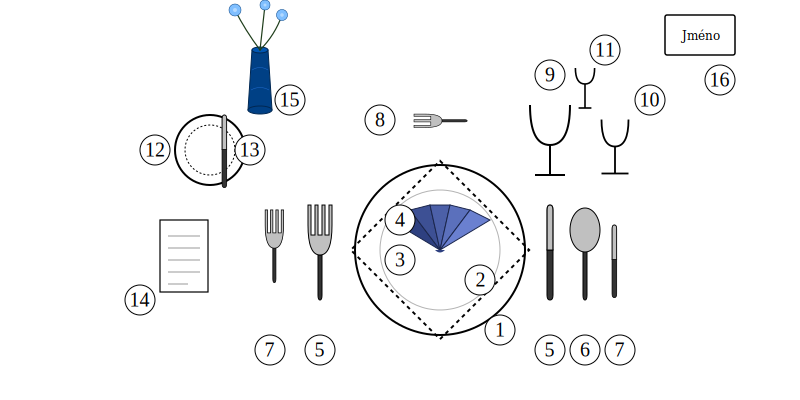
\includegraphics[width=0.9\textwidth]{images/couvert.png}
    \caption{Nákres couvertu}
    \label{fig:couvert}
\end{figure}
\begin{enumerate}
    \item Klubový talíř
    \item Masový příbor
    \item Předkrmový příbor
    \item Předkrmový příbor
    \item Polévková lžíce
    \item Pečivový talířek
    \item Sklenice na víno k hlavnímu chodu
    \item Sklenice na víno k předkrmu
    \item Sklenice na likér k dezertu
    \item Ubrousek
    \item Dezertní vidlička
    \item Masový talíř
\end{enumerate}


% -----------------------------------------------------------------------------
% 10. Charakteristika menu
% -----------------------------------------------------------------------------
\subsection{Charakteristika celého menu}
Menu ke křtinám je navrženo tak, aby postupně gradovalo od lehkých chutí až po sytější hlavní chod, zakončený sladkou tečkou.\\

\textbf{Amuse bouche} (Kanapka s parmskou šunkou a melounem) - spojení sladkého a slaného. Jemná, slaná chuť sušené šunky kontrastuje s melounem.\\

\textbf{Studený předkrm} (Bruschetta s rajčaty a mozzarellou) - barvy trikolóry, křupavá opečená bagetka potřená česnekem, doplněná šťavnatými rajčaty, krémovou mozzarellou a čerstvou bazalkou.\\

\textbf{Teplý předkrm} ( Dýňové raviolky) - Jemné těstoviny plněné sladkavou dýní, často doplněné šalvějovým máslem nebo parmazánem. Elegantní a moderní\\

\textbf{Polévka} (Hovězí vývar s játrovými knedlíčky) - Základ české slavnostní tabule, Symbolizuje rodinnou pohodu a tradici. \\

\textbf{Hlavní chod} (Kuřecí roláda na bylinkách s pečenými bramborami ve slupce) - Díky kuřecímu maso je chod lehký, ale bylinky mu dodávají výraznou vůni\\

\textbf{Dezert} (Vanilkové cupcakes) - Nadýchané těsto s výraznou chutí vanilky a jemným krémem \\
\newpage
% -----------------------------------------------------------------------------
% 11. Žádanka na inventář   
% -----------------------------------------------------------------------------
\subsection{Žádanka na inventář}

\begin{tabular}{|c|c|c|}
\hline
\textbf{Druh} & \textbf{Popis} & \textbf{Množství} \\
\hline
Textilní & Ubrus bílý x*y & 1\\
& Příručník & 1\\
& Molton bílý & 1\\
& Dečka pod talíř & 2\\
Kovové & Masový nůž & 2\\
& Dezertní vidlička & 2\\
& Polévková lžíce & 2\\
& Masová vidlička & 2\\
& Předkrmová vidlička & 2\\
& Předkrmový nůž & 2\\
Sklo & Sklenice na víno k hlavnímu chodu & 2\\
& Sklenice na víno k předkrmu & 2\\
& Sklenice na likér k dezertu & 2\\
Porcelán & Klubový talíř & 2\\
& Terina & 1\\
& Pečivový talířek & 2\\
& Masový talíř & 2\\
Ostatní & Ikebana & 1\\
& Plato & 1\\
& Keridon & 1\\
\hline
\end{tabular}
\end{document}